\subsection{Utilizations of the re module}
\label{sec:utilizations}

\noindent \textbf{Utilization}: A \emph{utilization} occurs whenever a regex is used in source code.  We detect utilizations by statically analyzing source code and recording calls to the {\tt re} module in Python.

\subsubsection{Utilization defined}
\label{sec:utilizationDefined}
Within a Python source code file, a {utilization} of the {\tt re} module is composed of a function, a pattern, and 0 or more flags.  Figure~\ref{fig:exampleUsage} presents an example of one {utilization}, with key components labeled. The function call is {\tt re.compile}, \verb!"(0|-?[1-9][0-9]*)$"! is the pattern, and {\tt re.MULTILINE} is an (optional) flag. When executed, this {utilization}  will compile a regex into the variable {\tt r1} from the pattern \verb!"(0|-?[1-9][0-9]*)$"!.  The resulting regex \cverb!(0|-?[1-9][0-9]*)$! is composed of two regex fragments: \cverb!0! and \cverb!-?[1-9][0-9]*! operated on by the OR \verb!|!, and contained in a CG \verb!(! \verb!)! so that the following the END feature (\cverb!$!) applies regardless of which fragment is matched. Because of the {\tt re.MULTILINE} flag used, the END specifies a position at the end of every line (instead of only the end of the last line).

\begin{figure}[tb]
\centering
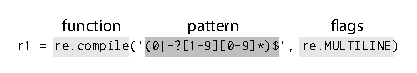
\includegraphics[width=.8\textwidth]{nontex/illustrations/exampleUsage.eps}
\vspace{-12pt}
\caption{Example of one regex utilization}
\vspace{-6pt}
\label{fig:exampleUsage}
\end{figure}

The regex fragment \cverb!0! matches \verb!"0"!, and the fragment on the right of the OR,
\\*\cverb!-?[1-9][0-9]*!, matches all positive or negative integers (not starting with 0) like \verb!"123"!, \verb!"9"!, \verb!"-10000"! or \verb!"-8"!. When combined the full regex \cverb!(0|-?[1-9][0-9]*)$! matches all positive and negative integers at the end of lines.  For example the multi-line string: \verb!"line 1: xyz 85!\gverb!\n!\verb!line2: -2!\gverb!\n!\verb!last line!\gverb!\n!\verb!"! will match at the end of the first two lines.  Expressing zero or one dash characters using the regex fragment \cverb!-?! is useful so that the sign of the integer will be part of the capture, (e.g., from \verb!"A: -9!\gverb!\n!\verb!"!, \verb!"-9"! is captured, not just \verb!"9"!).

\noindent \textbf{Pattern}: A \emph{pattern} is extracted from a utilization, as shown in Figure~\ref{fig:exampleUsage}. As described in Section~\ref{sec:featureOverview}, a pattern specifies a series of regular expression language feature tokens which can be compiled by an engine into a regex.  A regex compiled from the pattern in Figure~\ref{fig:exampleUsage} .

Note that because the vast majority of regular expression features are shared across most general programming languages (e.g., Java, C, C\#, or Ruby), a Python pattern will (almost always) behave the same when used in other languages as mentioned in Section~\ref{sec:usuallyOk}, whereas a utilization is not universal in the same way (i.e., it is very unlikely to compile in other languages because of variations in programming language syntax and the names of functions).

\subsubsection{Omission of calls to compiled regexes}
Every utilization recorded using the technique described in Appendix~\ref{app:miningImplementation} is an invocation directly using the {\tt re} library, like {\tt re.compile(...)} or {\tt re.search(...)}.  However, this technique does not record calls on compiled objects.  For example the regex described in Section~\ref{sec:utilizationDefined} is stored in the variable {\tt r1}, and a function call on that variable like {\tt r1.search("-45")} is not recorded.  However, this omission only impacts the interpretation of Figure~\ref{fig:partFunctions}, which describes which function calls were observed (calls to compiled objects are excluded).  This issue does not impact the coverage of patterns, because every compiled regex like {\tt r1} comes from a call to {\tt re.compile(...)}, which is captured by the technique used in this study.

\subsubsection{Selecting projects to mine for utilizations}
\label{sec:selectingProjects}

The goal of this experiment was to collect regexes from a variety of projects to represent the breadth of how developers use the language features.  In order to obtain utilizations from a pseudo-random, broad selection of projects, \dbfetch{nProjScanned} projects containing Python code were mined for utilizations as described in Appendix~\ref{app:miningImplementation}.  This section describes how these projects were selected.

Every time a new repository is created on GitHub, a new unique identifier (strictly greater than existing identifiers) is generated and assigned to that repository.  This work refers to these identifiers using the shorthand: \emph{repoID}.  At the time the mining for utilizations used in this study was performed, the largest repoID was between 32 million and 33 million.  Dividing these repoIDs into four groups each of size $2^{23} = 8,388,608$ (with the fourth group being a little larger than that), the second group, which spans the range 8,388,608 - 16,777,215 was split into 32 sections so that starting indices were 262,144 repoIDs apart.  The original intention was to mine the entire second $1/4$ of the first 32 million repo IDs, but due to the challenges described in Appendix~\ref{app:miningChallenges}, only the first 100 or so projects from each of the 32 starting points was mined.  Instead of spending the majority of available time on perfecting a mining technique, the determination was made to analyze the data that had already been gathered.

\subsubsection{Observed utilizations of the re module}

\begin{table}[tb]
\begin{center}
\begin{small}
\caption{How saturated are projects with utilizations? (RQ2)}
\label{table:saturation}

\begin{tabular}{l|ccccc}
\toprule
source & Q1 & Avg & Med & Q3 & Max \\
 \midrule \bigstrut
utilizations per project & 2 & 32 & 5 & 19 & 1,427 \\
 \midrule \bigstrut
files per project & 2 & 53 & 6 & 21 & 5,963 \\
 \midrule \bigstrut
utilizing files per project & 1 & 11 & 2 & 6 & 541 \\
 \midrule \bigstrut
utilizations per file & 1 & 2 & 1 & 3 & 207 \\
\bottomrule
\end{tabular}
\end{small}
\end{center}
\vspace{-12pt}
\end{table}


\paragraph{Saturation of artifacts with regexes.} Out of the \dbfetch{nProjScanned}\ projects scanned, \dbfetch{percentProjectsUsingRegex}\% (\dbfetch{nProjectsUsingRegex}) contained at least one utilization.  Within a project, a duplicate utilization was marked when two versions of the same file have the same function, pattern and flags.  In total, \dbfetch{nUsages} non-duplicate utilizations were observed.  To illustrate how saturated projects are with regexes, measurements are made for the number of utilizations per project, number of files scanned per project, number of files containing utilizations, and number of utilizations  per file, as shown in Table~\ref{table:saturation}.

Of projects containing at least one utilization, the average utilizations per project was 32 and the maximum  was 1,427.  The project with the most utilizations is a C\# project\footurl{https://github.com/Ouroboros/Arianrhod} that maintains a collection of source code for 20 Python libraries, including larger libraries like {\tt pip}, {\tt celery} and {\tt ipython}.  These larger Python libraries contain many utilizations.
From Table~\ref{table:saturation}, it can also be seen that each project had an average of 11 files containing any utilization, and each of these files had an average of 2 utilizations.

\begin{figure}[ht]
\centering
  \centering
  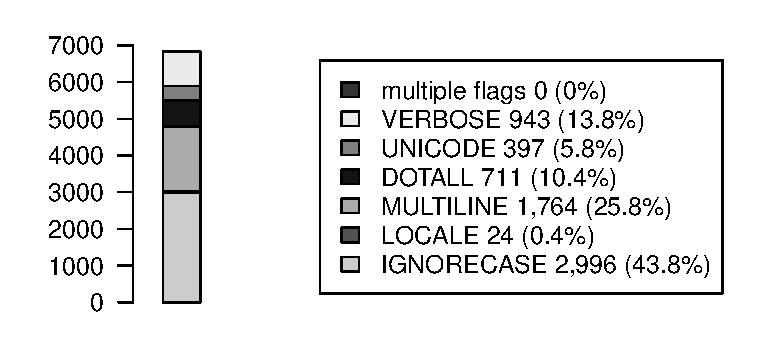
\includegraphics[width=.72\textwidth]{nontex/illustrations/partFlags.eps}
  \caption{Which behavioral flags are used?}
  \vspace{-6pt}
\label{fig:partFlags}
\end{figure}

\begin{figure}[ht]
\centering
  \centering
  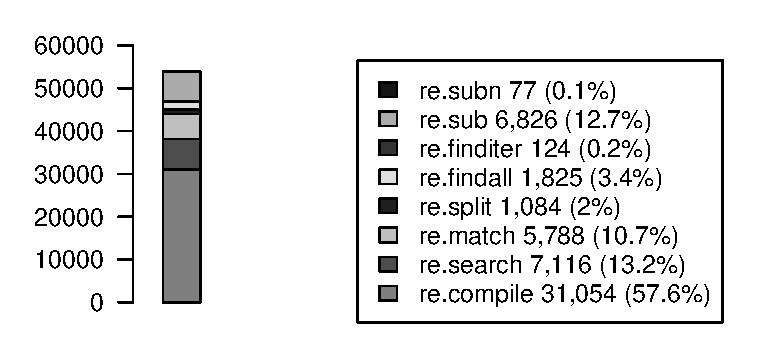
\includegraphics[width=.70\textwidth]{nontex/illustrations/partFunctions.eps}
  \caption{Which behavioral flags are used?}
  \vspace{-6pt}
\label{fig:partFunctions}
\end{figure}

\paragraph{Flags and functions.}
\label{sec:flagsAndFunctions} As shown in figure ~\ref{fig:partFlags}, of all behavioral flags used, ignorecase (\DTLfetch{data}{key}{percentI}{value}\%) and multiline (\DTLfetch{data}{key}{percentM}{value}\%) were the most frequently used.  It is also worth noting that although multiple flags can be combined using a bitwise or, this was never observed.
When considering flag use, non-behavioral flags (default and debug) were excluded, which are present in \DTLfetch{data}{key}{percentFlags0}{value}\% of all \emph{utilizations}.

As seen in Figure~\ref{fig:partFunctions} The `compile' function encompasses \DTLfetch{data}{key}{percentCompile}{value}\% of all utilizations.  Regexes may be compiled in an attempt to improve performance (only compile once) or to abstract the regex from the rest of the code.  Compiled regexes are often observed at the top of a file, listed along with other highly-scoped variables maintained separately from blocks of code.  Using the other {\tt re} module functions in-line may be less preferred by developers because of the `magic strings' which could be refactored to a variable.
\pagebreak
